% Options for packages loaded elsewhere
\PassOptionsToPackage{unicode}{hyperref}
\PassOptionsToPackage{hyphens}{url}
\PassOptionsToPackage{dvipsnames,svgnames,x11names}{xcolor}
%
\documentclass[journal=,manuscript=]{achemso}
\usepackage[version=3]{mhchem}
\newcommand*\mycommand[1]{\texttt{\emph{#1}}}



\usepackage{amsmath,amssymb}
\usepackage{iftex}
\ifPDFTeX
  \usepackage[T1]{fontenc}
  \usepackage[utf8]{inputenc}
  \usepackage{textcomp} % provide euro and other symbols
\else % if luatex or xetex
  \usepackage{unicode-math}
  \defaultfontfeatures{Scale=MatchLowercase}
  \defaultfontfeatures[\rmfamily]{Ligatures=TeX,Scale=1}
\fi
\usepackage{lmodern}
\ifPDFTeX\else  
    % xetex/luatex font selection
\fi
% Use upquote if available, for straight quotes in verbatim environments
\IfFileExists{upquote.sty}{\usepackage{upquote}}{}
\IfFileExists{microtype.sty}{% use microtype if available
  \usepackage[]{microtype}
  \UseMicrotypeSet[protrusion]{basicmath} % disable protrusion for tt fonts
}{}
\makeatletter
\@ifundefined{KOMAClassName}{% if non-KOMA class
  \IfFileExists{parskip.sty}{%
    \usepackage{parskip}
  }{% else
    \setlength{\parindent}{0pt}
    \setlength{\parskip}{6pt plus 2pt minus 1pt}}
}{% if KOMA class
  \KOMAoptions{parskip=half}}
\makeatother
\usepackage{xcolor}
\setlength{\emergencystretch}{3em} % prevent overfull lines
\setcounter{secnumdepth}{5}
% Make \paragraph and \subparagraph free-standing
\ifx\paragraph\undefined\else
  \let\oldparagraph\paragraph
  \renewcommand{\paragraph}[1]{\oldparagraph{#1}\mbox{}}
\fi
\ifx\subparagraph\undefined\else
  \let\oldsubparagraph\subparagraph
  \renewcommand{\subparagraph}[1]{\oldsubparagraph{#1}\mbox{}}
\fi

\usepackage{color}
\usepackage{fancyvrb}
\newcommand{\VerbBar}{|}
\newcommand{\VERB}{\Verb[commandchars=\\\{\}]}
\DefineVerbatimEnvironment{Highlighting}{Verbatim}{commandchars=\\\{\}}
% Add ',fontsize=\small' for more characters per line
\usepackage{framed}
\definecolor{shadecolor}{RGB}{241,243,245}
\newenvironment{Shaded}{\begin{snugshade}}{\end{snugshade}}
\newcommand{\AlertTok}[1]{\textcolor[rgb]{0.68,0.00,0.00}{#1}}
\newcommand{\AnnotationTok}[1]{\textcolor[rgb]{0.37,0.37,0.37}{#1}}
\newcommand{\AttributeTok}[1]{\textcolor[rgb]{0.40,0.45,0.13}{#1}}
\newcommand{\BaseNTok}[1]{\textcolor[rgb]{0.68,0.00,0.00}{#1}}
\newcommand{\BuiltInTok}[1]{\textcolor[rgb]{0.00,0.23,0.31}{#1}}
\newcommand{\CharTok}[1]{\textcolor[rgb]{0.13,0.47,0.30}{#1}}
\newcommand{\CommentTok}[1]{\textcolor[rgb]{0.37,0.37,0.37}{#1}}
\newcommand{\CommentVarTok}[1]{\textcolor[rgb]{0.37,0.37,0.37}{\textit{#1}}}
\newcommand{\ConstantTok}[1]{\textcolor[rgb]{0.56,0.35,0.01}{#1}}
\newcommand{\ControlFlowTok}[1]{\textcolor[rgb]{0.00,0.23,0.31}{#1}}
\newcommand{\DataTypeTok}[1]{\textcolor[rgb]{0.68,0.00,0.00}{#1}}
\newcommand{\DecValTok}[1]{\textcolor[rgb]{0.68,0.00,0.00}{#1}}
\newcommand{\DocumentationTok}[1]{\textcolor[rgb]{0.37,0.37,0.37}{\textit{#1}}}
\newcommand{\ErrorTok}[1]{\textcolor[rgb]{0.68,0.00,0.00}{#1}}
\newcommand{\ExtensionTok}[1]{\textcolor[rgb]{0.00,0.23,0.31}{#1}}
\newcommand{\FloatTok}[1]{\textcolor[rgb]{0.68,0.00,0.00}{#1}}
\newcommand{\FunctionTok}[1]{\textcolor[rgb]{0.28,0.35,0.67}{#1}}
\newcommand{\ImportTok}[1]{\textcolor[rgb]{0.00,0.46,0.62}{#1}}
\newcommand{\InformationTok}[1]{\textcolor[rgb]{0.37,0.37,0.37}{#1}}
\newcommand{\KeywordTok}[1]{\textcolor[rgb]{0.00,0.23,0.31}{#1}}
\newcommand{\NormalTok}[1]{\textcolor[rgb]{0.00,0.23,0.31}{#1}}
\newcommand{\OperatorTok}[1]{\textcolor[rgb]{0.37,0.37,0.37}{#1}}
\newcommand{\OtherTok}[1]{\textcolor[rgb]{0.00,0.23,0.31}{#1}}
\newcommand{\PreprocessorTok}[1]{\textcolor[rgb]{0.68,0.00,0.00}{#1}}
\newcommand{\RegionMarkerTok}[1]{\textcolor[rgb]{0.00,0.23,0.31}{#1}}
\newcommand{\SpecialCharTok}[1]{\textcolor[rgb]{0.37,0.37,0.37}{#1}}
\newcommand{\SpecialStringTok}[1]{\textcolor[rgb]{0.13,0.47,0.30}{#1}}
\newcommand{\StringTok}[1]{\textcolor[rgb]{0.13,0.47,0.30}{#1}}
\newcommand{\VariableTok}[1]{\textcolor[rgb]{0.07,0.07,0.07}{#1}}
\newcommand{\VerbatimStringTok}[1]{\textcolor[rgb]{0.13,0.47,0.30}{#1}}
\newcommand{\WarningTok}[1]{\textcolor[rgb]{0.37,0.37,0.37}{\textit{#1}}}

\providecommand{\tightlist}{%
  \setlength{\itemsep}{0pt}\setlength{\parskip}{0pt}}\usepackage{longtable,booktabs,array}
\usepackage{calc} % for calculating minipage widths
% Correct order of tables after \paragraph or \subparagraph
\usepackage{etoolbox}
\makeatletter
\patchcmd\longtable{\par}{\if@noskipsec\mbox{}\fi\par}{}{}
\makeatother
% Allow footnotes in longtable head/foot
\IfFileExists{footnotehyper.sty}{\usepackage{footnotehyper}}{\usepackage{footnote}}
\makesavenoteenv{longtable}
\usepackage{graphicx}
\makeatletter
\def\maxwidth{\ifdim\Gin@nat@width>\linewidth\linewidth\else\Gin@nat@width\fi}
\def\maxheight{\ifdim\Gin@nat@height>\textheight\textheight\else\Gin@nat@height\fi}
\makeatother
% Scale images if necessary, so that they will not overflow the page
% margins by default, and it is still possible to overwrite the defaults
% using explicit options in \includegraphics[width, height, ...]{}
\setkeys{Gin}{width=\maxwidth,height=\maxheight,keepaspectratio}
% Set default figure placement to htbp
\makeatletter
\def\fps@figure{htbp}
\makeatother

\makeatletter
\@ifpackageloaded{caption}{}{\usepackage{caption}}
\AtBeginDocument{%
\ifdefined\contentsname
  \renewcommand*\contentsname{Table of contents}
\else
  \newcommand\contentsname{Table of contents}
\fi
\ifdefined\listfigurename
  \renewcommand*\listfigurename{List of Figures}
\else
  \newcommand\listfigurename{List of Figures}
\fi
\ifdefined\listtablename
  \renewcommand*\listtablename{List of Tables}
\else
  \newcommand\listtablename{List of Tables}
\fi
\ifdefined\figurename
  \renewcommand*\figurename{Figure}
\else
  \newcommand\figurename{Figure}
\fi
\ifdefined\tablename
  \renewcommand*\tablename{Table}
\else
  \newcommand\tablename{Table}
\fi
}
\@ifpackageloaded{float}{}{\usepackage{float}}
\floatstyle{ruled}
\@ifundefined{c@chapter}{\newfloat{codelisting}{h}{lop}}{\newfloat{codelisting}{h}{lop}[chapter]}
\floatname{codelisting}{Listing}
\newcommand*\listoflistings{\listof{codelisting}{List of Listings}}
\makeatother
\makeatletter
\makeatother
\makeatletter
\@ifpackageloaded{caption}{}{\usepackage{caption}}
\@ifpackageloaded{subcaption}{}{\usepackage{subcaption}}
\makeatother
\ifLuaTeX
  \usepackage{selnolig}  % disable illegal ligatures
\fi
\usepackage{bookmark}

\IfFileExists{xurl.sty}{\usepackage{xurl}}{} % add URL line breaks if available
\urlstyle{same} % disable monospaced font for URLs
\hypersetup{
  pdftitle={La Palma Earthquakes Mechanism},
  pdfauthor={Steve Purves; Rowan Cockett},
  pdfkeywords={La Palma, Earthquakes},
  colorlinks=true,
  linkcolor={blue},
  filecolor={Maroon},
  citecolor={Blue},
  urlcolor={Blue},
  pdfcreator={LaTeX via pandoc}}

\author{Steve Purves}
\affiliation{ Curvenote,  }


\email{steve@curvenote.com}
\author{Rowan Cockett}
\affiliation{ Curvenote,  }




\keywords{La PalmaEarthquakes}

\title[]{La Palma Earthquakes Mechanism}
\makeatletter
\begin{document}
\maketitle
\begin{abstract}
In September 2021, a significant jump in seismic activity on the island
of La Palma (Canary Islands, Spain) signaled the start of a volcanic
crisis that still continues at the time of writing. Earthquake data is
continually collected and published by the Instituto Geográphico
Nacional (IGN). \ldots{}
\end{abstract}

\section{Introduction}\label{introduction}

\textsubscript{Source:
\href{https://voidmain443.github.io/example_manuscriptquarto/index.ipynb.html}{Article
Notebook}}

\textsubscript{Source:
\href{https://voidmain443.github.io/example_manuscriptquarto/index.ipynb.html}{Article
Notebook}}

\begin{Shaded}
\begin{Highlighting}[]
\NormalTok{plt.figure(figsize}\OperatorTok{=}\NormalTok{(}\DecValTok{6}\NormalTok{, }\DecValTok{1}\NormalTok{))}
\NormalTok{plt.eventplot(eruptions, lineoffsets}\OperatorTok{=}\DecValTok{0}\NormalTok{, linelengths}\OperatorTok{=}\FloatTok{0.1}\NormalTok{, color}\OperatorTok{=}\StringTok{\textquotesingle{}black\textquotesingle{}}\NormalTok{)}
\NormalTok{plt.gca().axes.get\_yaxis().set\_visible(}\VariableTok{False}\NormalTok{)}
\NormalTok{plt.ylabel(}\StringTok{\textquotesingle{}\textquotesingle{}}\NormalTok{)}
\NormalTok{plt.show()}
\end{Highlighting}
\end{Shaded}

\begin{figure}[H]

\centering{

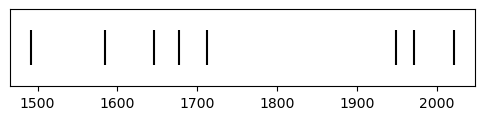
\includegraphics{index_files/figure-pdf/fig-timeline-output-1.png}

}

\caption{\label{fig-timeline}Timeline of recent earthquakes on La Palma}

\end{figure}%

\textsubscript{Source:
\href{https://voidmain443.github.io/example_manuscriptquarto/index.ipynb.html}{Article
Notebook}}

\textsubscript{Source:
\href{https://voidmain443.github.io/example_manuscriptquarto/index.ipynb.html}{Article
Notebook}}

Based on data up to and including 1971, eruptions on La Palma happen
every 79.8 years on average.

\textsubscript{Source:
\href{https://voidmain443.github.io/example_manuscriptquarto/index.ipynb.html}{Article
Notebook}}

Studies of the magma systems feeding the volcano, such as
\citet{marrero2019}, have proposed that there are two main magma
reservoirs feeding the Cumbre Vieja volcano; one in the mantle (30-40km
depth) which charges and in turn feeds a shallower crustal reservoir
(10-20km depth).

A prior study of the magma systems feeding the volcano proposed that
there are two main magma reservoirs feeding the Cumbre Vieja volcano
\citep{marrero2019} .

\textsubscript{Source:
\href{https://voidmain443.github.io/example_manuscriptquarto/index.ipynb.html}{Article
Notebook}}

Eight eruptions have been recorded since the late 1400s
(Figure~\ref{fig-timeline}).

\textsubscript{Source:
\href{https://voidmain443.github.io/example_manuscriptquarto/index.ipynb.html}{Article
Notebook}}

Data and methods are discussed in Section~\ref{sec-data-methods}.

\textsubscript{Source:
\href{https://voidmain443.github.io/example_manuscriptquarto/index.ipynb.html}{Article
Notebook}}

Let \(x\) denote the number of eruptions in a year. Then, \(x\) can be
modeled by a Poisson distribution

\begin{equation}\phantomsection\label{eq-poisson}{
p(x) = \frac{e^{-\lambda} \lambda^{x}}{x !}
}\end{equation}

where \(\lambda\) is the rate of eruptions per year. Using
Equation~\ref{eq-poisson}, the probability of an eruption in the next
\(t\) years can be calculated.

\textsubscript{Source:
\href{https://voidmain443.github.io/example_manuscriptquarto/index.ipynb.html}{Article
Notebook}}

\begin{longtable}[]{@{}ll@{}}
\caption{Recent historic eruptions on La
Palma}\label{tbl-history}\tabularnewline
\toprule\noalign{}
Name & Year \\
\midrule\noalign{}
\endfirsthead
\toprule\noalign{}
Name & Year \\
\midrule\noalign{}
\endhead
\bottomrule\noalign{}
\endlastfoot
Current & 2021 \\
Teneguía & 1971 \\
Nambroque & 1949 \\
El Charco & 1712 \\
Volcán San Antonio & 1677 \\
Volcán San Martin & 1646 \\
Tajuya near El Paso & 1585 \\
Montaña Quemada & 1492 \\
\end{longtable}

Table~\ref{tbl-history} summarises the eruptions recorded since the
colonization of the islands by Europeans in the late 1400s.

\textsubscript{Source:
\href{https://voidmain443.github.io/example_manuscriptquarto/index.ipynb.html}{Article
Notebook}}

\begin{figure}

\centering{

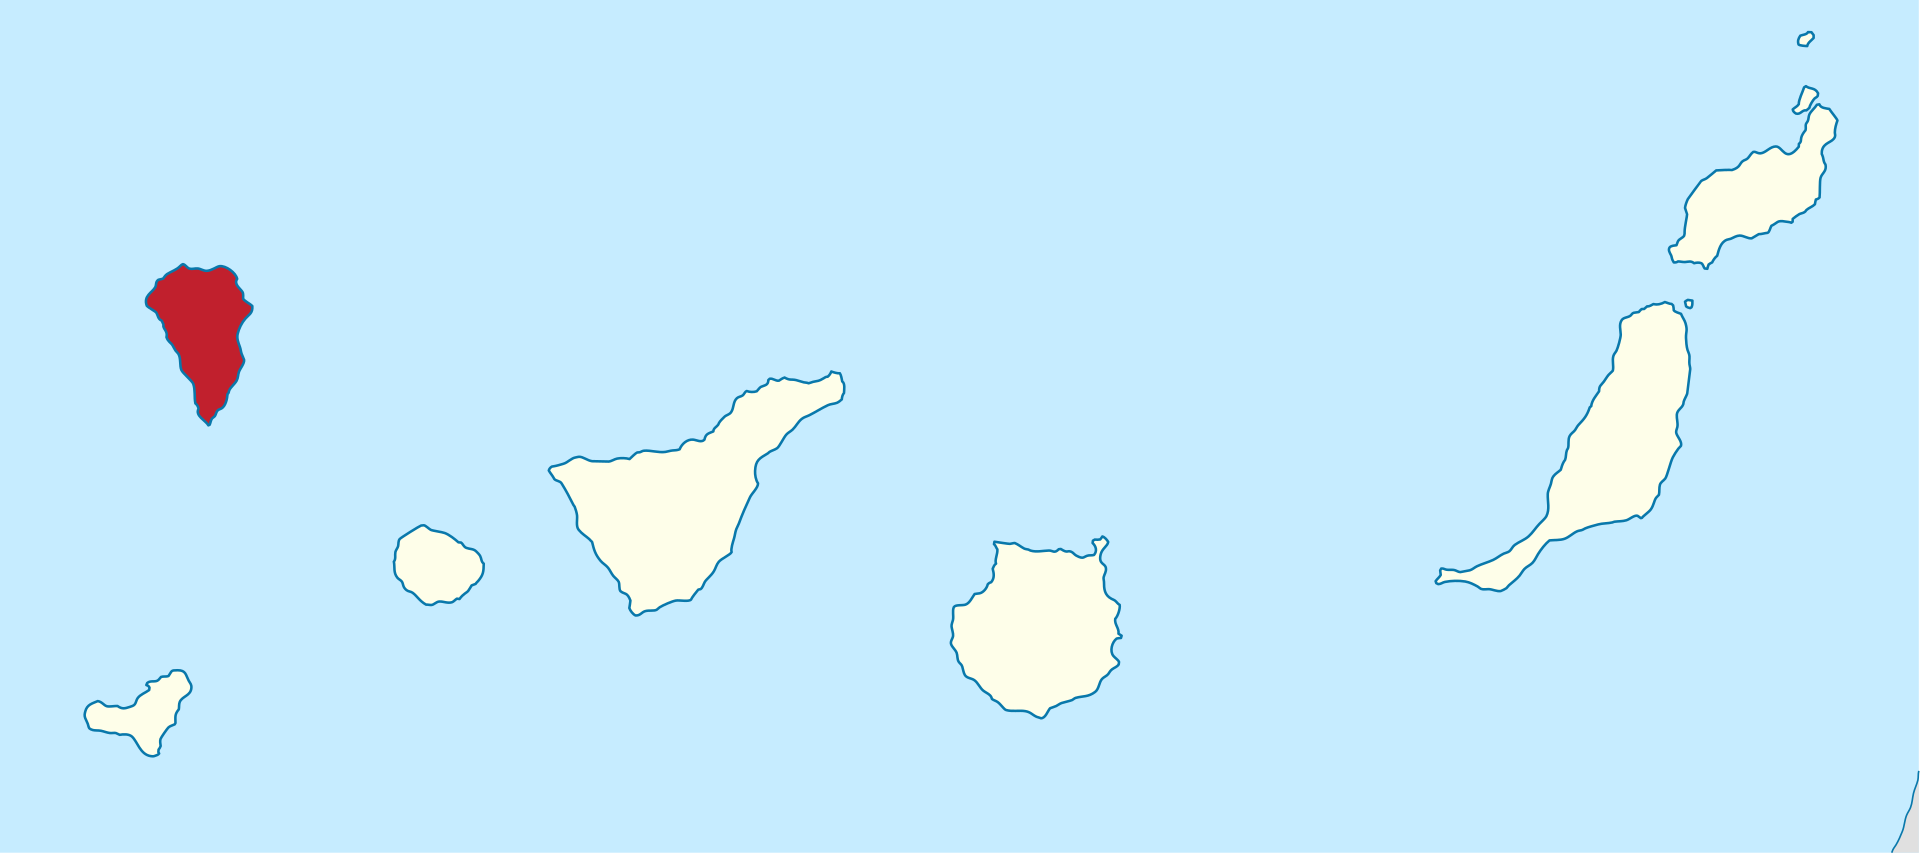
\includegraphics{images/la-palma-map.png}

}

\caption{\label{fig-map}Map of La Palma}

\end{figure}%

La Palma is one of the west most islands in the Volcanic Archipelago of
the Canary Islands (Figure~\ref{fig-map}).

\textsubscript{Source:
\href{https://voidmain443.github.io/example_manuscriptquarto/index.ipynb.html}{Article
Notebook}}

\begin{figure}[H]

\centering{

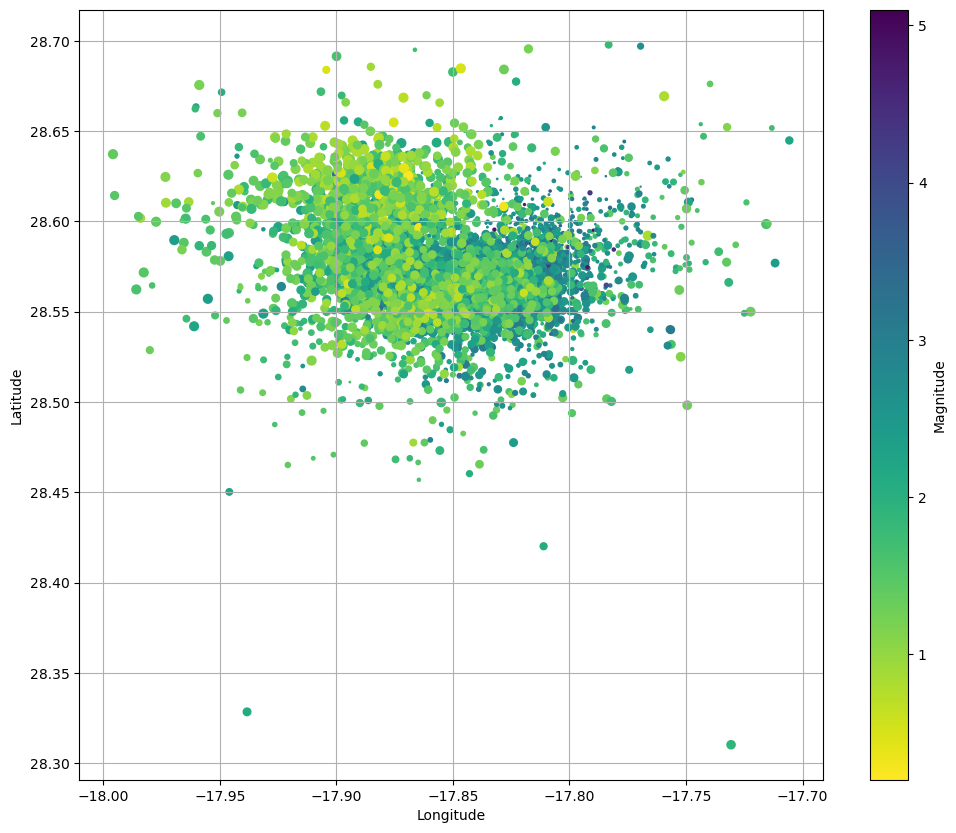
\includegraphics{index_files/figure-latex/notebooks-data-screening-fig-spatial-plot-output-1.png}

}

\caption{\label{fig-spatial-plot}Locations of earthquakes on La Palma
since 2017.}

\end{figure}%

\textsubscript{Source:
\href{https://voidmain443.github.io/example_manuscriptquarto/index.ipynb.html}{Article
Notebook}}

Figure~\ref{fig-spatial-plot} shows the location of recent Earthquakes
on La Palma.

\textsubscript{Source:
\href{https://voidmain443.github.io/example_manuscriptquarto/index.ipynb.html}{Article
Notebook}}

\section{Data \& Methods}\label{sec-data-methods}

\textsubscript{Source:
\href{https://voidmain443.github.io/example_manuscriptquarto/index.ipynb.html}{Article
Notebook}}

Data and methods are discussed in Section~\ref{sec-data-methods}

\textsubscript{Source:
\href{https://voidmain443.github.io/example_manuscriptquarto/index.ipynb.html}{Article
Notebook}}

\section{Conclusion}\label{conclusion}

\textsubscript{Source:
\href{https://voidmain443.github.io/example_manuscriptquarto/index.ipynb.html}{Article
Notebook}}

\section*{References}\label{references}
\addcontentsline{toc}{section}{References}

\textsubscript{Source:
\href{https://voidmain443.github.io/example_manuscriptquarto/index.ipynb.html}{Article
Notebook}}


  \bibliography{references.bib}


\end{document}
